% !TEX root = ../Dokumentation.tex
\subsection{Elektronisches Layout}
Damit über den Mikrocontroller auf die einzelnen elektrischen Komponenten zugegriffen und mit ihnen kommuniziert werden kann, werden diese miteinander verbunden. Dazu werden sie auf eine Leiterplatte geführt welche auf den MCU gesteckt wird.
\\[0.2cm]

\textbf{PCB-Schaltung}\\[0.2cm]
Für die Leiterplatte wurde eine entsprechende Schaltung entworfen, die das Zusammenspiel der elektrischen Hardware ermöglicht. Dabei waren die technischen Spezifikationen der Teile ausschlaggebend für den Entwurf.
So musste beispielsweise gewährleistet werden, dass  keine zu hohen Spannungen auf den Mikrocontroller oder auf andere Komponente geführt werden. Für die Spannungsüberwachung der Akkumulatoren, wurde daher ein Spannungsteiler eingebaut. Mit diesem wird nicht das ganze Potential über den Mikrocontroller geführt, sondern nur ein Wert im vetragbaren Bereich. Bei den Motoren hingegen, wurden DC/DC-Wandler eingesetzt um die Spannung möglichst konstant auf 5V zu halten.
Die Schaltung wurde mithilfe des Altium Designer erstellt und das komplette Schema befindet sich im Anhang.
\\[0.2cm]
\begin{figure}[H]
\centering
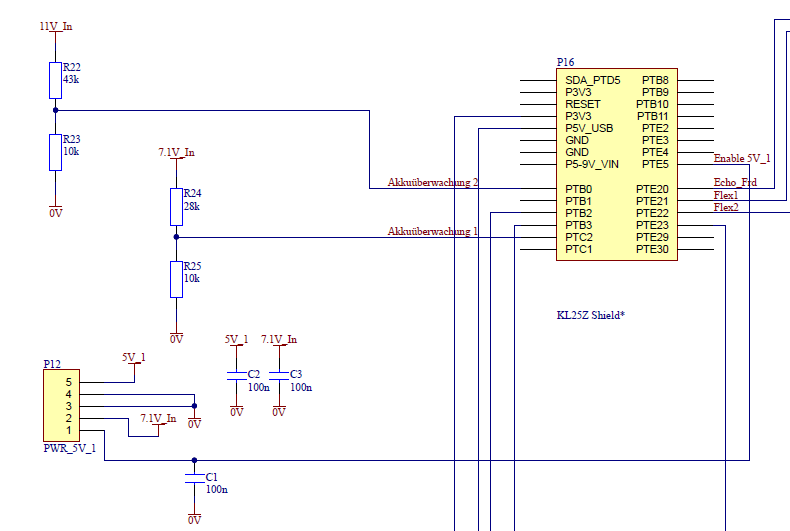
\includegraphics[width=0.5\textwidth]{03_Loesungskonzept/pictures/pcbspannungsteiler.png}
\caption{Ausschnitt aus dem Elektroschema}	
\end{figure}

\textbf{PCB-Layout}
\\[0.2cm]
Nach Anleitung des Elektroschemas, wurde die Platine entworfen. Dabei durften die vorgegebenen Werte der Maschinenbauabteilung für Länge und Breite nicht überschritten werden, damit die Platine an der vorgesehenen Position befestigt werden konnte. Anschliessend wurden die Footprints für die Elektrokomponenten wie Kondensatoren, Widerstände, etc. angeordnet. Dafür mussten diese zum Teil selbst gezeichnet werden, z.B für die Steckeranschlüsse, da in der Altium Bibliothek kein passendes Pendant zur Verfügung stand.
Nach der definitiven Positionierung, wurden die Leiterbahnen gezeichnet, um die jeweiligen Teile miteinander zu verbinden.
\\[0.2cm]
\begin{figure}[H]
\centering
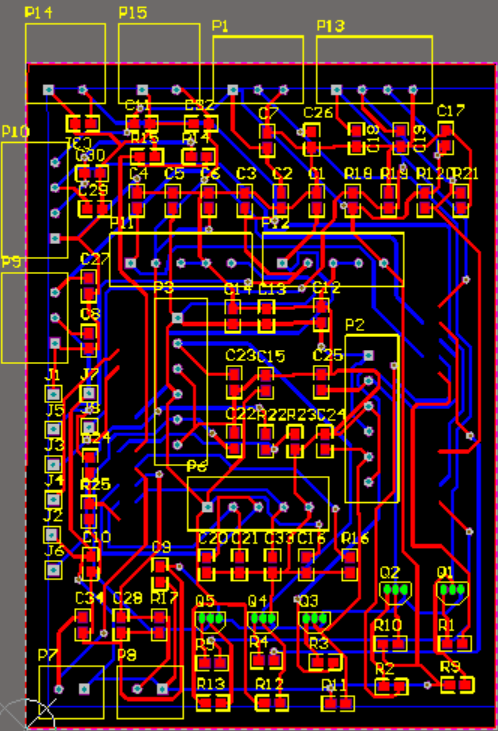
\includegraphics[width=0.5\textwidth]{03_Loesungskonzept/pictures/pcb_print.png}
\caption{PCB}	
\end{figure}
\textbf{Vergleich Konzept und Umsetzung}\\[0.2cm]
Die Umsetzung gestaltete sich ziemlich genau wie vorgesehen. Jedoch wurde im Pren1 noch keine konkretes Konzept für die Leiterplatte erstellt, daher gab es auch keine grossen Änderungen in der Umsetzung.
